\newcommand{\paragraphit}[1] {\paragraph{\textit{#1}}}

\renewcommand{\hbAppendixPrefix}{B}

\renewcommand{\thefigure}{\hbAppendixPrefix\arabic{figure}}
\setcounter{figure}{0}
\renewcommand{\thetable}{\hbAppendixPrefix\arabic{table}}
\setcounter{table}{0}
\renewcommand{\theequation}{\hbAppendixPrefix\arabic{equation}}
\setcounter{equation}{0}

\section{Supplementary Material 2 for Chapter 3}


%\documentclass{article}
%\usepackage{supmaterial}
%
%\title{Supplementary File S1 \\
%	\large Multiobjective Strain Design: A Framework for Modular Cell Engineering}
%
%\author[1,2]{Sergio Garcia}
%\author[1,2,*]{Cong T. Trinh}
%\affil[1]{Department of Chemical and Biomolecular Engineering, The University of Tennessee, Knoxville, TN}
%\affil[2]{Center for Bioenergy Innovation, Oak Ridge National Laboratory, Oak Ridge, TN}
%\affil[*]{Corresponding author: Tel: 865-974-2181. Email: ctrinh@utk.edu.}
%
%\begin{document}
%{\let\newpage\relax\maketitle}
%\tableofcontents
%\newpage

\subsection{Solution method: Multiobjective Evolutionary Algorithm}

\subsubsection{Definitions}
\paragraph{Terms}
\begin{description}
\item[Parent network:] A parent network is a metabolic model of a host organism that is used to construct a modular cell.
\item[Production module:] A production module is a metabolic pathway that is added to a modular cell to synthesize a target product.
\item[Production network:] A production network is a combination of a parent network and a production module.
\item[MOEA:] Multiobjective evolutionary algorithm.
\end{description}

\paragraph{Sets}
\begin{description}
\item[$\mathcal{I}_k:$] Set of metabolite indices in production network $k$.
\item[$\mathcal{J}_k:$] Set of reaction indices in production network $k$.
\item[$\mathcal{K}:$] Set of production network indices.
\item[$\mathcal{C}$]: Set of candidate reaction deletion indices, where $\mathcal{C} \subseteq \mathcal{J}^{parent} \subseteq \mathcal{J}_k \;, \forall k \in \mathcal{K}$.
\end{description}

\paragraph{Continuous variables}
\begin{description}
\item[$v_{jk}:$] Flux of reaction $j$ in production network $k$.
\item[$v_{Pk}:$] Flux of target product (P) reaction in production network $k$.
\item[$v_{Xk}:$] Flux of biomass (X) synthesis reaction in production network $k$.
\item[$f_k:$] Objective function for production network $k$.
\item[$f_k^{wGCP}:$] \textit{wGCP} objective function for production network $k$.
\item[$f_k^{sGCP}:$] \textit{sGCP} objective function for production network $k$.
\item[$f_k^{NGP}:$] \textit{NGP} objective function for production network $k$.
\item[$p_k:$] Penalty objective function for production network k.
\item[$q^{enum}:$] Objective function for enumerating alternative solutions.
\end{description}

\paragraph{Binary variables}
\begin{description}
\item[$y_j:$] Reaction deletion indicator that takes a value of 0 if reaction $j$ is deleted in a modular cell, and 1 otherwise.
\item[$z_{jk}:$] Endogeonous, module-specific reaction indicator that takes a value of 1 if reaction $j$ is added back to the production module in network $k$, and 0 otherwise.
\item[$d_{jk}= y_j \lor z_{jk}:$] Modeling variable which takes a value of 1 if reaction $j$ may carry flux in production network $k$, and 0 otherwise.
\end{description}

\paragraph{Parameters}
\begin{description}
\item[$S_{ijk}:$] Stoichiometric coefficient of metabolite $i$ in reaction $j$ of production network $k$.
\item[$l_{jk}:$] Lower bound flux for reaction $j$ in production network $k$.
\item[$u_{jk}:$] Upper bound flux for reaction $j$ in production network $k$.
\item[$\alpha:$] Maximum number of deletion reactions in a modular cell.
\item[$\beta_k:$] Maximum number of endogenous module-specific reactions in the module of production network $k$.
\item[$\epsilon:$] Small scalar used for tilting the biomass objective function to obtain the minimum product rate available at the maximum growth rate. In the simulation, we used $\epsilon=0.0001$.
\end{description}

\subsubsection{Solver} \label{sec:mainMOP}
We used the \textit{gamultiobj()} solver, an implementation of NSGA-II \citep{deb2002}, from the MATLAB Optimization Toolbox to solve our combinatorial multiobjective optimization, formulated as an unconstrained multiobjective problem of
the form:
\begin{equation}
\max (p_1,p_2,\dots ,p_{|\mathcal{K}|})^T
\end{equation}
with a \textit{bitstring} population type where each individual is a binary vector corresponding to the design variables $y_j$ (reaction deletions) and $z_{jk}$ (endogenous module-specific reactions). To enforce the constraints on the number of deletion and endogenous module reactions, a penalty function $p_k$, instead of $f_k$, (Section \ref{sec:penalty}) and customized genetic operators (Section \ref{sec:customOp}) were used, respectively. %The design objective values are computed during the MOEA objective function evaluation by solving the associated linear programs ((\ref{eq:rpgLP}) for wGCP, and additionally  (\ref{eq:rpngLP}) for sGCP).

\subsubsection{Penalty Objective function} \label{sec:penalty}

To restrict the maximum number of reaction deletions, we optimized the following penalty function $p_k$ instead of $f_k$:

\begin{equation} \label{eq:pkp}
p_k =
\begin{dcases}
\frac{f_k}{\displaystyle \sum_{j\in C} (1-y_j)} & \text{if}\;  \sum_{j\in C} (1-y_j) > \alpha\\
f_k & \text{otherwise}
\end{dcases}
\end{equation}
The penalty function is designed to decrease $f_k$ of an individual proportionally to the number of deletion reactions exceeding the set limit $\alpha$. Implementation of this penalty function helps the  optimization problem converge rapidly because favorable deletion reaction candidates are likely kept to obtain desirable solutions. After simulation, only solutions satisfying the maximum reaction deletion constraint are preserved to obtain the Pareto set of our original problem.

\subsubsection{Design objective computation} \label{sec:design_obj_comp}
Depending on desirable applications, the following design objectives are considered:
\begin{alignat}{3}
	f_k^{wGCP} & =\frac{v_{Pk}^{\mu}}{v_{P_{max}k}^{\mu}}\in[0,1], \qquad & & \forall k\in \mathcal{K} \label{eq:obj_wgcp}\\
	f_k^{sGCP} & =\frac{v_{Pk}^{\mu}}{v_{P_{max}k}^{\mu}} \, \frac{v_{Pk}^{\bar{\mu}}}{v_{P_{max}k}^{\bar{\mu}}} \in[0,1], \;  & &  \forall k\in \mathcal{K} \label{eq:obj_sgcp}\\
	f_k^{NGP} & = \frac{v_{Pk}^{\bar{\mu}}}{v_{P_{max}k}^{\bar{\mu}}} \in[0,1], \qquad  & &  \forall k\in \mathcal{K} \label{eq:obj_ngp}
	\end{alignat}

%The design objectives  (\ref{eq:obj_wgcp})-(\ref{eq:obj_ngp}) feature product and biomass metabolic fluxes at key cellular states. These fluxes are determined using steady-state constraint based models of metabolism. Each target product is represented by a separate model. Depending on the design objective, additional constraints must be imposed to the model, such as the need for cell growth, or the absence of cell growth. First, we present the space of steady-state reaction fluxes of production network $k$, when a minimum amount of cell growth is required:

\noindent In \eqref{eq:obj_wgcp}-\eqref{eq:obj_ngp}, the terms $v_{Pk}^{\mu}$, $v_{P_{max}k}^{\mu}$, $v_{Pk}^{\bar{\mu}}$, and $v_{P_{max}k}^{\bar{\mu}}$ are computed by solving the following linear programming problems:

\begin{alignat}{3}
& v_{Pk}^{\mu} 	&\in& \,	\text{arg }	\underset{}{\text{max}} \{v_{Xk}-\epsilon v_{Pk} : v_k\in \Pi_k^{\mu}(d_{jk})	\} \label{eq:rpgLP}	\\
& v_{P_{max}k}^{\mu} &\in& \,	\text{arg }	\underset{}{\text{max}} \{v_{Pk} : v_k\in \Pi_k^{\mu} (d_{jk} = 1, \; \forall j\in \mathcal{J}_k) 	\}   \label{eq:vpmaxLP_g}	\\
& v_{Pk}^{\bar{\mu}} 	&\in& \,	\text{arg }	\underset{}{\text{min}} \{v_{Pk} : v_k\in \Pi_k^{\bar{\mu}}(d_{jk})\} \label{eq:rpngLP} \\
& v_{P_{max}k}^{\bar{\mu}}&\in& \,	 \text{arg }	\underset{}{\text{max}} \{v_{Pk} : v_k\in \Pi_k^{\bar{\mu}}(d_{jk} = 1, \; \forall j\in \mathcal{J}_k)\}  \label{eq:vpmaxLP_ng}
\end{alignat}
The maximum product synthesis fluxes in \eqref{eq:vpmaxLP_g} and \eqref{eq:vpmaxLP_ng}, used to normalize the design objectives in \eqref{eq:obj_wgcp}-\eqref{eq:obj_ngp}, only need to be computed once for each network prior to solving the multiobjective problem (MOP).

In $\eqref{eq:rpgLP}-\eqref{eq:vpmaxLP_ng}, \Pi_k^{\mu}$ is the space of steady-state reaction fluxes of production network $k$ where a minimum cell growth is required, defined as follows:

\begin{alignat}{2}
	\nonumber	& \Pi_k^{\mu} (d_{jk}):=\{v_{jk}\in\mathbb{R}\, \forall j \in \mathcal{J}_k: \\
		&\qquad	\sum_{j\in \mathcal{J}_k} S_{ijk} v_{jk} =0,  && \forall i\in \mathcal{I}_k 		\label{eq:piG1}\\
		&\qquad l_{jk}  \le v_{jk} \le u_{jk},  && \forall j\in \mathcal{J}_k 					\label{eq:piG2}\\
		&\qquad l_{jk} d_{jk} \le v_{jk} \le u_{jk} d_{jk}, && \forall j\in \mathcal{C} 	\label{eq:piG3}\\
		&\qquad v_{Xk} \ge \text{minimum growth rate}		\label{eq:piG6} \}
\end{alignat}

\noindent Constraints (\ref{eq:piG1})-(\ref{eq:piG2}) correspond to mass balance and flux bounds, as described in the main text. Constraint (\ref{eq:piG3}) ensures that reaction $j$ cannot carry any flux, if it is deleted in the modular cell and not present in module $k$.  Constraint \eqref{eq:piG6} specifies any minimum growth rate requirement.

When the design goals involve the stationary phase \eqref{eq:rpngLP}-\eqref{eq:vpmaxLP_ng}, the space of steady-state reaction fluxes for production network $k$, $\Pi_k^{\bar{\mu}}$, is defined as follows:

\begin{alignat}{2}
	\nonumber	& \Pi_k^{\bar{\mu}}(d_{jk}):=\{v_{jk}\in\mathbb{R}\, \forall j \in \mathcal{J}_k: \\
		&\qquad	\sum_{j\in \mathcal{J}_k} S_{ijk} v_{jk} =0,  && \forall i\in \mathcal{I}_k 		\label{eq:piNG1}\\
		&\qquad l_{jk}  \le v_{jk} \le u_{jk},  && \forall j\in \mathcal{J}_k 					\label{eq:piNG2}\\
		&\qquad l_{jk} d_{jk} \le v_{jk} \le u_{jk} d_{jk}, && \forall j\in \mathcal{C} 	\label{eq:piNG3}\\
		&\qquad v_{Xk} = 0	\label{eq:piNG6} \}
\end{alignat}

If any of the linear programs associated with $f_k$ becomes infeasible, i.e., $\Pi_k^{\mu}=\emptyset \; \text{or}\; \Pi_k^{\bar{\mu}}=\emptyset$, then $f_k$ is set to $0$.
\subsubsection{Termination criteria}
We implemented a non-domination termination criterion to determine when simulation must stop to retrieve a solution, as described in Algorithm~\ref{alg:1}.

\begin{algorithm}
		\caption{Non-domination termination criterion for MOEA. PF: Pareto front, PS: Pareto set.} \label{alg:1}
	\DontPrintSemicolon
	[PF, PS] = solveMOP(initialPoint = $\emptyset$, 	stall\_generations, ...) \;
	total\_generations = 0 \;
	\Do{\upshape{ \textbf{any}}(PF \textbf{dominates} PF\_old) \textbf{and} total\_generations \textbf{$\le$} max\_total\_generations \textbf{and} run\_time \textbf{$\le$} {max\_run\_time} }{
		PF\_old = PF \;
		PS\_old = PS \;
		[PF, PS] = solveMOP(initialPoint = PS\_old, 	stall\_generations, ...) \;
		total\_generations = total\_generations + stall\_generations \;
	}
\end{algorithm}

Based on this criterion, the solution is retrieved if new non-dominated solutions cannot be found for a predefined number of stall generations. For our study, we used highly conservative, empirical values of 500 and 1000 stall generations with runtime limits of 1-2h and 10-15h for core and genome scale models, respectively.

\subsubsection{Customized genetic operators to handle endogenous module-specific reactions} \label{sec:customOp}
We modified the default scattered crossover and uniform mutation operators of \textit{gamultiobj()} to enforce the constraint on the number of endogenous module reactions and improve convergence. First, we ensured both crossover and mutation operators to produce only individuals that meet the maximum module reaction constraint, i.e., $\sum_{j \in \mathcal{J}_k} z_{jk} \le \beta_k, \; \forall k \in \mathcal{K}$. Next, we required that only reactions deleted in the modular cell can be used as endogenous module-specific reactions, i.e., $z_{jk} \le 1- y_j, \; \forall j \in \mathcal{J}, \, k \in \mathcal{K}$. Finally, we specified the crossover operator to perform crossover on the variables associated with reaction deletions and endogenous module reactions separately, for each production network.

\subsubsection{Parameters} \label{sec:MOPparameters}
All MOEA parameters, except the population size, were left as default. In our study, we set the empirically conservative values for population sizes of 200 and 400 for core and genome-scale models to converge in 2 h and 15 h of simulation time, respectively.



%TODO: FIX runaway
\subsubsection{Enumeration of alternative solutions}
If a solution $w$ produces the same objective vector as a Pareto optimal solution $x^*$, i.e., $f(w)=f(x^*)$ and $w \ne x^*$, we say that $w$ constitutes an alternative solution of $x^*$. To enumerate alternative solutions for a specific Pareto optimal design, we iteratively solve a minimization problem of the form:
\begin{equation}
\min q^{enum}
\end{equation}
\noindent using MATLAB's genetic algorithm \textit{ga()}. Using the Jaccard similarity metric\footnote{The Jaccard similarity between vectors $r$ and $s$, $\textbf{jacc}(r,s)$,  corresponds to the fraction of common elements between $r$ and $s$. If $r$ and $s$ are the same, the Jaccard similarity is 1; if both vectors do not share any elements, then it takes a value of 0.}, we define $q^{enum}$, which takes a value of 0 if an alternative solution is found, as follows:

\begin{numcases}{q^{enum}=}
M & \text {if}\; $ \{y_j:j\in \mathcal{J}_k\} \in \text{ExcludedSol}$\label{eq:enum1}\\
1-\textbf{jacc}(f^*,f) + \sum_{j\in \mathcal{C}} (1-y_j) & \text {if}\; $ \sum_{j \in \mathcal{C}} (1-y_j) > \alpha $\label{eq:enum2}\\
1-\textbf{jacc}(f^*,f) & \text{otherwise}\label{eq:enum3}
\end{numcases}

Initially, ExcludedSol will contain at least a target solution for which we are interested in finding alternative solutions. A large scalar $M$ is returned if the current set of deletions $\{y_j\}$ has been found previously, and hence cannot be an alternative solution \eqref{eq:enum1}. Likewise, a set of deletions $\{y_j\}$ may be a valid solution candidate but have more deletions than allowed \eqref{eq:enum2}. In that case, the negated Jaccard similarity is penalized according to the number of reaction deletions.

\subsubsection{Optimizing algorithm performance}

\paragraphit{Variable declaration.} To minimize the number of free variables in the optimization problem, we created binary variables, $y_j$, only for the reaction candidate set $C$ instead of all reactions in the parent model. Similarly, endogenous module reaction variables, $z_{jk}$, were only created for $j \in \mathcal{C}$ if $\beta_k >0$.

\paragraphit{Selection of starting population.} To accelerate convergence in our simulation, we used a predetermined starting population of individuals, if possible. A starting population can be derived from a previously obtained result; for instance, the solutions from $\alpha = 6$ can be used as a starting population to find solutions for $\alpha =7$. In some cases, we also used design strategies determined experimentally or orginated from other strain design algorithms (e.g., Optknock).
%
\paragraphit{Parallelization.} To increase the simulation speed, we performed the objective function computations  in parallel. This parallelization alleviated the bottlenecks of solving 1 linear programming problem (LP) in \textit{wGCP} (or \textit{NGP}) and 2 LPs in \textit{sGCP}.

\paragraphit{Archive of solutions.} Since computing objective functions is one critical bottleneck, we used a table (archive mapping design variables to design objectives) of previously evaluated individuals to avoid repeating this calculation. The size of the table is determined by the amount of memory available. For instance, we stored at most 50,000 solutions, which can be handled for 20 design objectives by a personal computer. When the table becomes full, it is erased to allow for higher quality individuals to be archived.


\subsection{Specifying the Set of Deletion Reaction Candidates for Manipulation} \label{sec:cand}

The set of deletion reaction candidates, \textit{C}, is a subset of all reactions in the parent network, excluding reactions infeasible to eliminate in practice and irrelevant to desirable phenotypes, as described below. Some criteria  used in \citep{feist2010} were adapted and implemented in our study.

	\paragraphit{ Macromolecule-associated reactions.} These reactions involve macromolecules whose biologically relevant roles are not well represented in the model (e.g., glycogen) or do not impact the optimal design of target product biosynthesis pathways. We identified macromolecule-associated reactions by screening metabolite IDs and formulas, for instance, those with total carbon number above 10 except currency metabolites (e.g., ATP, acetyl-CoA, etc.)

	\paragraphit{ Non-metabolic reactions.} These reactions belong to the functional categories such as ion transport, tRNA charging, etc. We identified these non-metabolic reactions by screening the reaction-subsystem annotation in the parent network.

	\paragraphit{ Modeling reactions.} These reactions are sink reactions and/or reactions which are not well characterized. We identified the modeling reactions by screening reaction IDs and sbo terms in the parent network.

	\paragraphit{  Transport reactions.} These reactions involve metabolites transported across cellular compartments. Most of these reactions are not included in \textit{C} due to their unspecific annotation or non-enzymatic mechanisms except some well-annotated reactions such as ATP synthase or NAD(P) transhydrogenase. We identified these transport reactions by screening metabolites appearing in multiple compartments.

	\paragraphit{ Exchange reactions.} These reactions are pseudo-reactions used to simulate steady-state conditions. We identified these reactions based on the characteristics they only have either substrates or products.

	\paragraphit{ Orphan reactions.} These reactions do not have known encoding enzymes. We determined them by screening gene-protein-reaction associations in the parent model.

	\paragraphit{ Essential reaction.} The essential reactions are the reactions whose removal from the model makes the maximum growth rate fall below the minimum acceptable value (i.e, 10-20\% of the predicted maximum growth rate). We identified these reactions by performing flux balance analysis combined with single reaction deletions.

	\paragraphit{ Blocked reactions.} These reactions carry a flux of 0 mmol/gCDW/hr across all production networks  (\hyperref[fig:candidaterxn]{Figure \ref{fig:candidaterxn}.A}).  We found these blocked reactions by performing flux variability analysis.

	\paragraphit{ Reactions in fully correlated sets (co-sets).} Sets of reactions that have linearly correlated fluxes are classified as co-sets. These reactions can belong to a linear pathway or more than one associated pathways. For each co-set, only one potential candidate reaction is needed to be considered in the reaction deletion candidate set. In our analysis, we considered all co-sets present in a master network, containing all production modules, to prevent potentially useful reaction deletions to be excluded from the candidate set (\hyperref[fig:candidaterxn]{Figure \ref{fig:candidaterxn}.B}). We found the co-sets by flux coupling analysis.

	\paragraphit{Special consideration for NGP designs.} The NGP design objective does not involve the growth phase, unlike wGCP and sGCP. Thus, the set of reaction deletion candidates for NGP designs are determined as outlined above except: i) essential reactions that should be considered in the candidate set and ii) blocked reactions that are determined under non-growth conditions (i.e. biomass flux is constrained to be 0).

\begin{figure}[ht]
    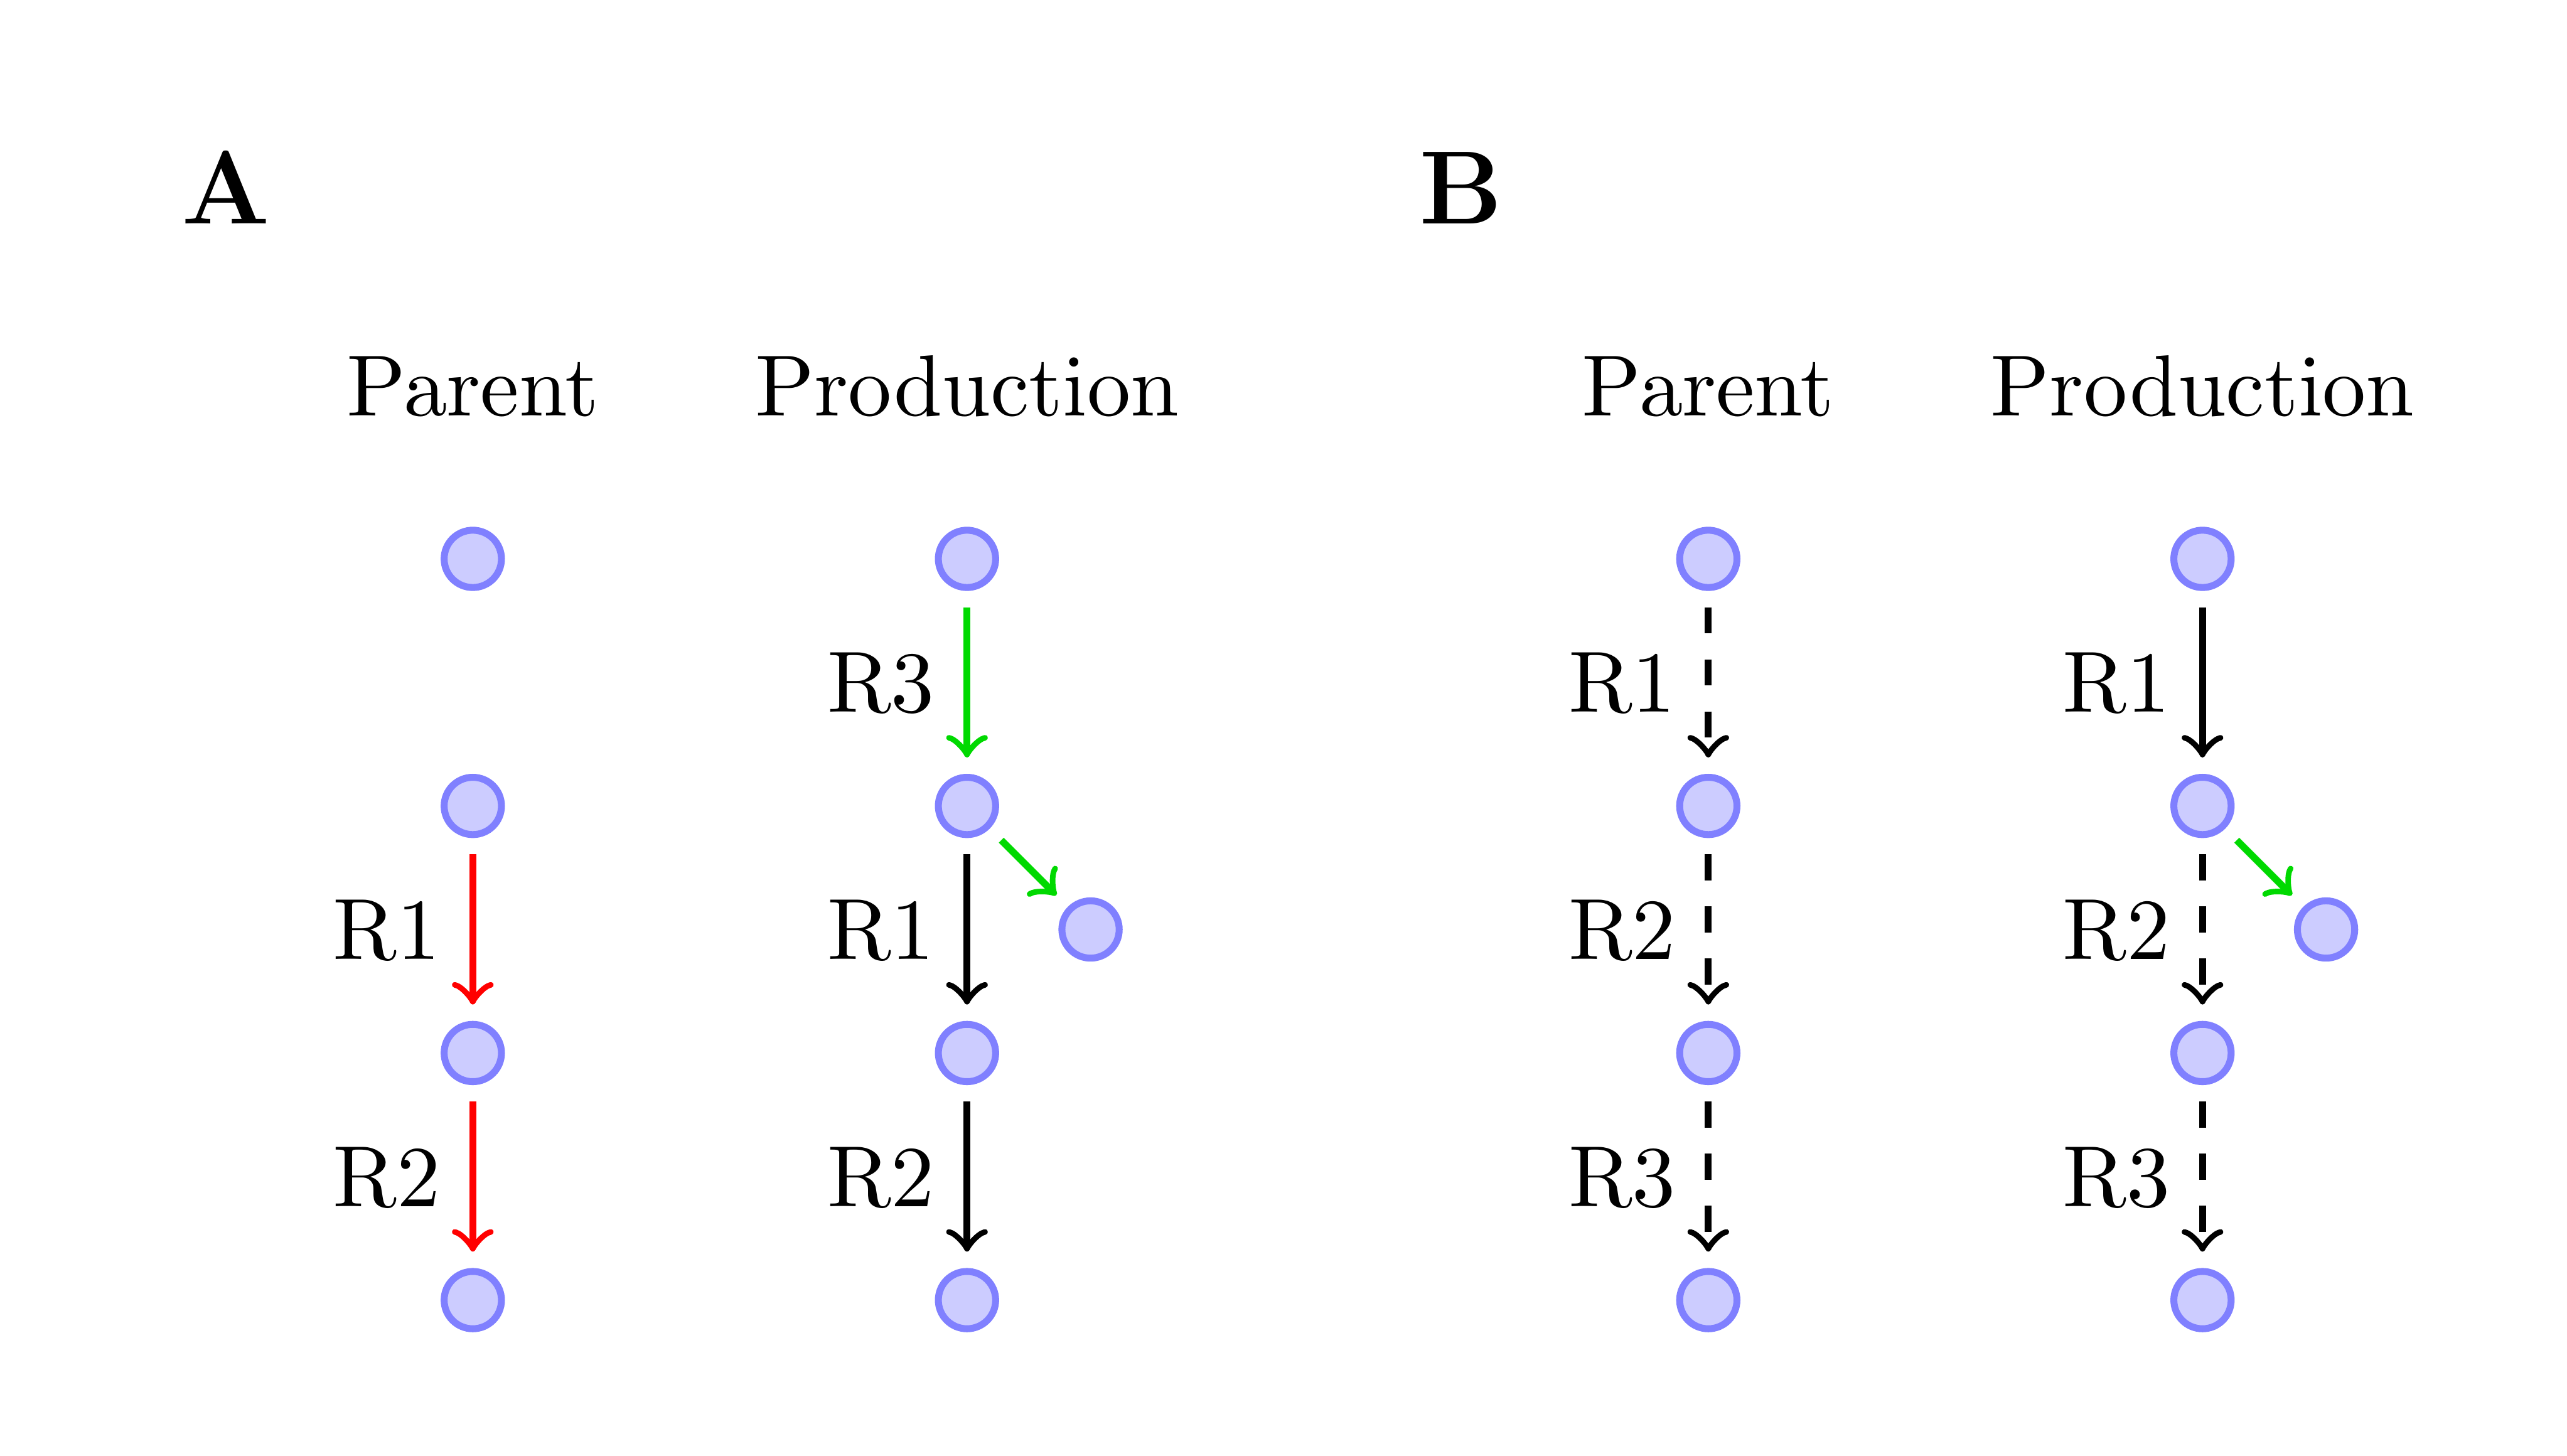
\includegraphics[width=.8\textwidth]{ms1-sm2-f1}
    \caption[Blocked and co-set reactions in deletion candidate determination]{(A.) Blocked reactions. The red arrows represent reactions originally blocked in the parent model, because the substrate of R1 cannot be produced. When heterologus reactions (green arrows) are added to produce a target chemical, the originally blocked reactions may become active and drain an intermediate of the production pathway. (B.) Reaction co-sets. The dashed arrows are used to indicated a fully correlated set. The addition of heterologous reactions (green arrows), alters the co-set definition and has important effect in deletion candidates. If R1 is considered as a deletion candidate, instead of R2 or R3, that would prevent the elimination of a potentially undesired pathway.}
\label{fig:candidaterxn}
\end{figure}
